\documentclass[12pt,a4paper,notitlepage]{article}
\usepackage{polski}
\usepackage[utf8]{inputenc} 
\usepackage[T1]{fontenc}
\usepackage[top=2cm, bottom=2cm, left=3cm, right=3cm]{geometry}
\usepackage{graphics}
\usepackage{gensymb}
\usepackage[pdftex]{graphicx}
\makeatletter
\newcommand{\linia}{\rule{\linewidth}{0.4mm}}
\renewcommand{\maketitle}{\begin{titlepage}
    \vspace*{1cm}
    \begin{center}\small
    Politechnika Wrocławska\\
    Wydział Podstawowych Problemów Techniki\\
    Systemy Wbudowane - Projekt
    \end{center}
    \vspace{3cm}
    \noindent\linia
    \begin{center}
      \LARGE \textsc{\@title}
         \end{center}
     \linia
    \vspace{0.5cm}
    \begin{flushright}
    \begin{minipage}{5cm}
    \textit{\small Autorzy:}\\
    \normalsize \textsc{\@author} \par
    \end{minipage}
    \vspace{5cm}
     \end{flushright}
    \vspace*{\stretch{6}}
    \begin{center}
    \@date
    \end{center}
  \end{titlepage}
}
\makeatother
\author{Grzegorz Stasiak\\Krzysztof Pająk}
\title{Automat do przygotowywania i gotowania zup}
\begin{document}

\maketitle
\tableofcontents
\newpage

\section{Problem i rozwiązanie}
\subsection{Zalety oraz wada samodzielnego gotowania}
Samodzielne przygotowywanie posiłków ma wiele zalet. Przede wszystkim pozwala na skomponowanie diety zależnej od własnych upodobań i potrzeb. Inną zaletą takiego przyrządzania dań jest mały koszt, w porównaniu na przykład z posiłkami podawanymi z restauracjach.\\ \\
Jednak znaczącą wadą takiego przyrządzania posiłków jest poświęcenie dużej ilości czasu na przygotowanie dania. Osoba gotująca spędza w kuchni conajmniej kilkanaście minut dziennie przy przyrządzaniu obiadu. Z tego też powodu wiele osób decyduje się na jedzenie w pośpiechu poza domem. Często jest to powodem niezdrowej diety czy dużych wydatków.

\subsection{Rozwiązanie problemu}
Idea automatu do przygotowywania i gotowania zup skupia się na problemie spędzania dużej ilości czasu w kuchni przy przygotowywaniu posiłków. Automat taki zaoszczędzałby czas przebyty w kuchni do minimum. Użytkownik musiałby jedynie włożyć składniki do odpowiednich pojemników i uruchomić urządzenie. Dzięki opcji zdalnego uruchamiania gotowania użytkownik mógłby, po uprzednim załadowaniu składników, uruchomić gotowanie zupy na przykład w czasie powrotu z pracy.\\ \\
Automat do przygotowywania i gotowania zup byłby także idealnym rozwiązaniem dla lokali gastronomicznych. Dzięki automatowi takie miejsca mogłyby przyspieszyć proces przygotowywania zup. 

\section{Funkcjonalność urządzenia}
\subsection{Spis funkcjonalności}
Poniżej znajduje się spis najważniejszych funkcjonalności automatu:
\begin{enumerate}
  \item Wybór przepisu spośród przepisów zapisanych w lokalnej bazie danych urządzenia lub spośród przepisów w internecie.
  \item Wyświetlenie instrukcji uzupełnienia pojemników na składniki.
  \item Sprawdzanie wagi umieszczonych składników.
  \item Manualne lub zdalne rozpoczęcie procesu gotowania.
  \item Automatyzacja procesu krojenia i siekania składników.
  \item Gotowanie ziemniaków/kaszy/makaronu.
  \item Wylanie niezdatnej do spożycia wody po gotowaniu do pojemnika na brudną wodę.
  \item Gotowanie zupy przez czas określony w przepisie.
  \item Sygnał dźwiękowy uruchamiany po zakończeniu procesu gotowania.
\end{enumerate}
Reszta funkcjonalności i zachowań poszczególnych komponentów znajduje się w rozdziale poświęconym komponentom.

\subsection{Wybór przepisu, lokalna oraz internetowa baza przepisów}
\subsubsection{Opis funkcjonalności}
Komputer posiada podłączoną kartę Micro-SD z bazą danych zawierającą początkowo kilkadziesiąt przepisów na zup. Użytkownik może za pomocą interfejsu wybrać interesujący go przepis i opcjonalnie wprowadzić niewielkie modyfikacje (na przykład określić ilość przypraw, gdy ma ich niewystarczająco wiele). Takie modyfikacje nie są zapisywane w bazie danych, ale są brane pod uwagę przed gotowaniem. Następnie użytkownik może rozpocząć kolejny etap, czyli uzupełnianie składników w pojemnikach.\\ \\
Urządzenie posiada też opcję połączenia ze stroną internetową producenta. Na tej stronie użytkownicy mogą tworzyć, modyfikować i umieszczać własne przepisy, które następnie są pobierane do urządzenia dzięki API. Po pobraniu przepisu istnieje możliwość zapisania go w pamięci urządzenia. Nowo utworzony w serwisie internetowym przepis musi być zatwierdzony przed administrację przed pojawieniem się publicznie.\\ \\
Urządzenie pozwala także na połączenie przez Internet z aplikacją mobilną, która pozwala na samodzielnie tworzenie oraz edycję przepisów. Aplikacja umożliwia także zdalne uruchomienie automatu.\\

\subsubsection{Format przepisu i bazy danych}
Przepis jest plikiem w formacie JSON, natomiast baza danych mieści się na karcie Micro-SD. W każdym z przepisów zawarte są informacje:
\begin{enumerate}
  \item Tytuł przepisu, autor, rodzaj: zupa dla jednej osoby, dla dwóch itd.
  \item Rodzaje składników, ich rozmieszczenie w pojemnikach oraz ilość.
  \item Rodzaje i ilość przypraw.
  \item Czas krojenia każdego ze składników w pojemniku
  \item Czas gotowania ziemniaków/kaszy/makaronu
  \item Optymalna temperatura wody.
  \item Czas gotowania zupy.
  \item Lista czynności do wykonania przez użytkownika.
\end{enumerate}

\subsubsection{Uszkodzony lub niepoprawny plik}
Jeżeli system nie zdołał poprawnie wczytać przepisu lub przepis zawiera niepoprawne wartości (na przykład ujemny czas gotowania) wtedy na głównym wyświetlaczu ukazuje się komunikat o błędzie. Komunikat proponuje oddanie urządzenia do serwisu ze względów bezpieczeństwa.\\ \\
Użytkownik może spróbować natomiast poradzić sobie z problemem na własną rękę. Należy wyłączyć urządzenie, zmienić kartę Micro-SD oraz ponownie uruchomić automat, co będzie skutkowało pustą bazą danych lecz odblokuje to normalne funkcje automatu.

\subsection{Wyświetlenie instrukcji uzupełnienia pojemników na składniki}
Użytkownik może zobaczyć intuicyjną instrukcję przygotowywania składników na główym wyświetlaczu urządzenia. Instrukcja jest generowana na podstawie pliku z przepisem (lub zapisana w pliku przepisu). Instrukcja zawiera takie informacje jak ilość poszczególnych składników, sugerowane miejsce ich rozłożenia. Równocześnie na wyświetlaczu są podawane komunikaty o błędach czy niewystarczającej ilości składników w pojemnikach. Komunikaty o błędach uniemożliwiają uruchomienie procesu gotowania/siekania, natomiast ostrzeżenia o np. braku niektórych składników mogą być pominięte.

\subsection{Sprawdzanie wagi umieszczonych składników}
Każdy z 9 pojemników na składniki zawiera niewielką wagę wbudowaną w spód pojemnika. Celem każdej z wag jest sprawdzanie ilości włożonych do pojemnika składników. Dane o wadze są wysyłane do głównego komputera, który odpowiada informacją, która jest wyświetlana na wyświetlaczy LCD pojemnika (na przykład: "Włożono 20/30g cebuli").

\subsection{Krojenie/siekanie składników w pojemnikach}
Automat posiada 9 specjalnych pojemników na składniki zupy. W środku 5 z nich zamontowane są niewielkie ostrza służące do pokrojenia składników na mniejsze kawałki, przykładowo marchwi, cebuli. Każdy z pojemników jest ponumerowany od 1 do 9. Przepis zawiera informację który składnik należy włożyć do którego pojemnika w jakiej ilości. Czas siekania za pomocą ostrzy w dla każdego z pojemników jest określony w pliku przepisu.

\subsection{Gotowanie wody/zupy oraz opróżnianie brudnej wody}
\subsubsection{Gotowanie ziemniaków, kaszy, makaronu czy ryżu}
Urządzenie posiada pojemnik na gotowanie ziemniaków, kaszy, makaronu lub ryżu. Pojemnik ten wyposażony jest w grzałkę, dzięki czemu woda w tym pojemniku może być ugotowana. Po ugotowaniu niezdatna do spożycia woda jest wylewana przewodami do specjalnego pojemnika na brudną wodę.

\subsubsection{Gotowanie zupy}
Urządzenie posiada drugi grzejnik, indukcyjny, który podgrzewa zupę w garnku. Jest to ostatni proces przygotowywania zupy, podgrzewane są wszystkie składniki znajdujące się razem w garnku.

\subsection{Sygnały dźwiękowe}
Po zakończeniu gotowania zupy urządzenie odtwarza w pętli co około pół minuty dźwięk informujący o zakończeniu procesu gotowania. Dźwięk odtwarza się do momentu zdjęcia garnka z grzejnika. Urządzenie sprawdza obecność garnka za pomocą wagi umieszczonej w podstawce na garnek.

\subsection{Przypomnienie o konieczności umycia pojemników}
Po zakończonym gotowaniu na głównym wyświetlaczu ukazuje się przypomnienie o umyciu garnków oraz pojemników na składniki.

\section{Diagram stanów urządzenia}

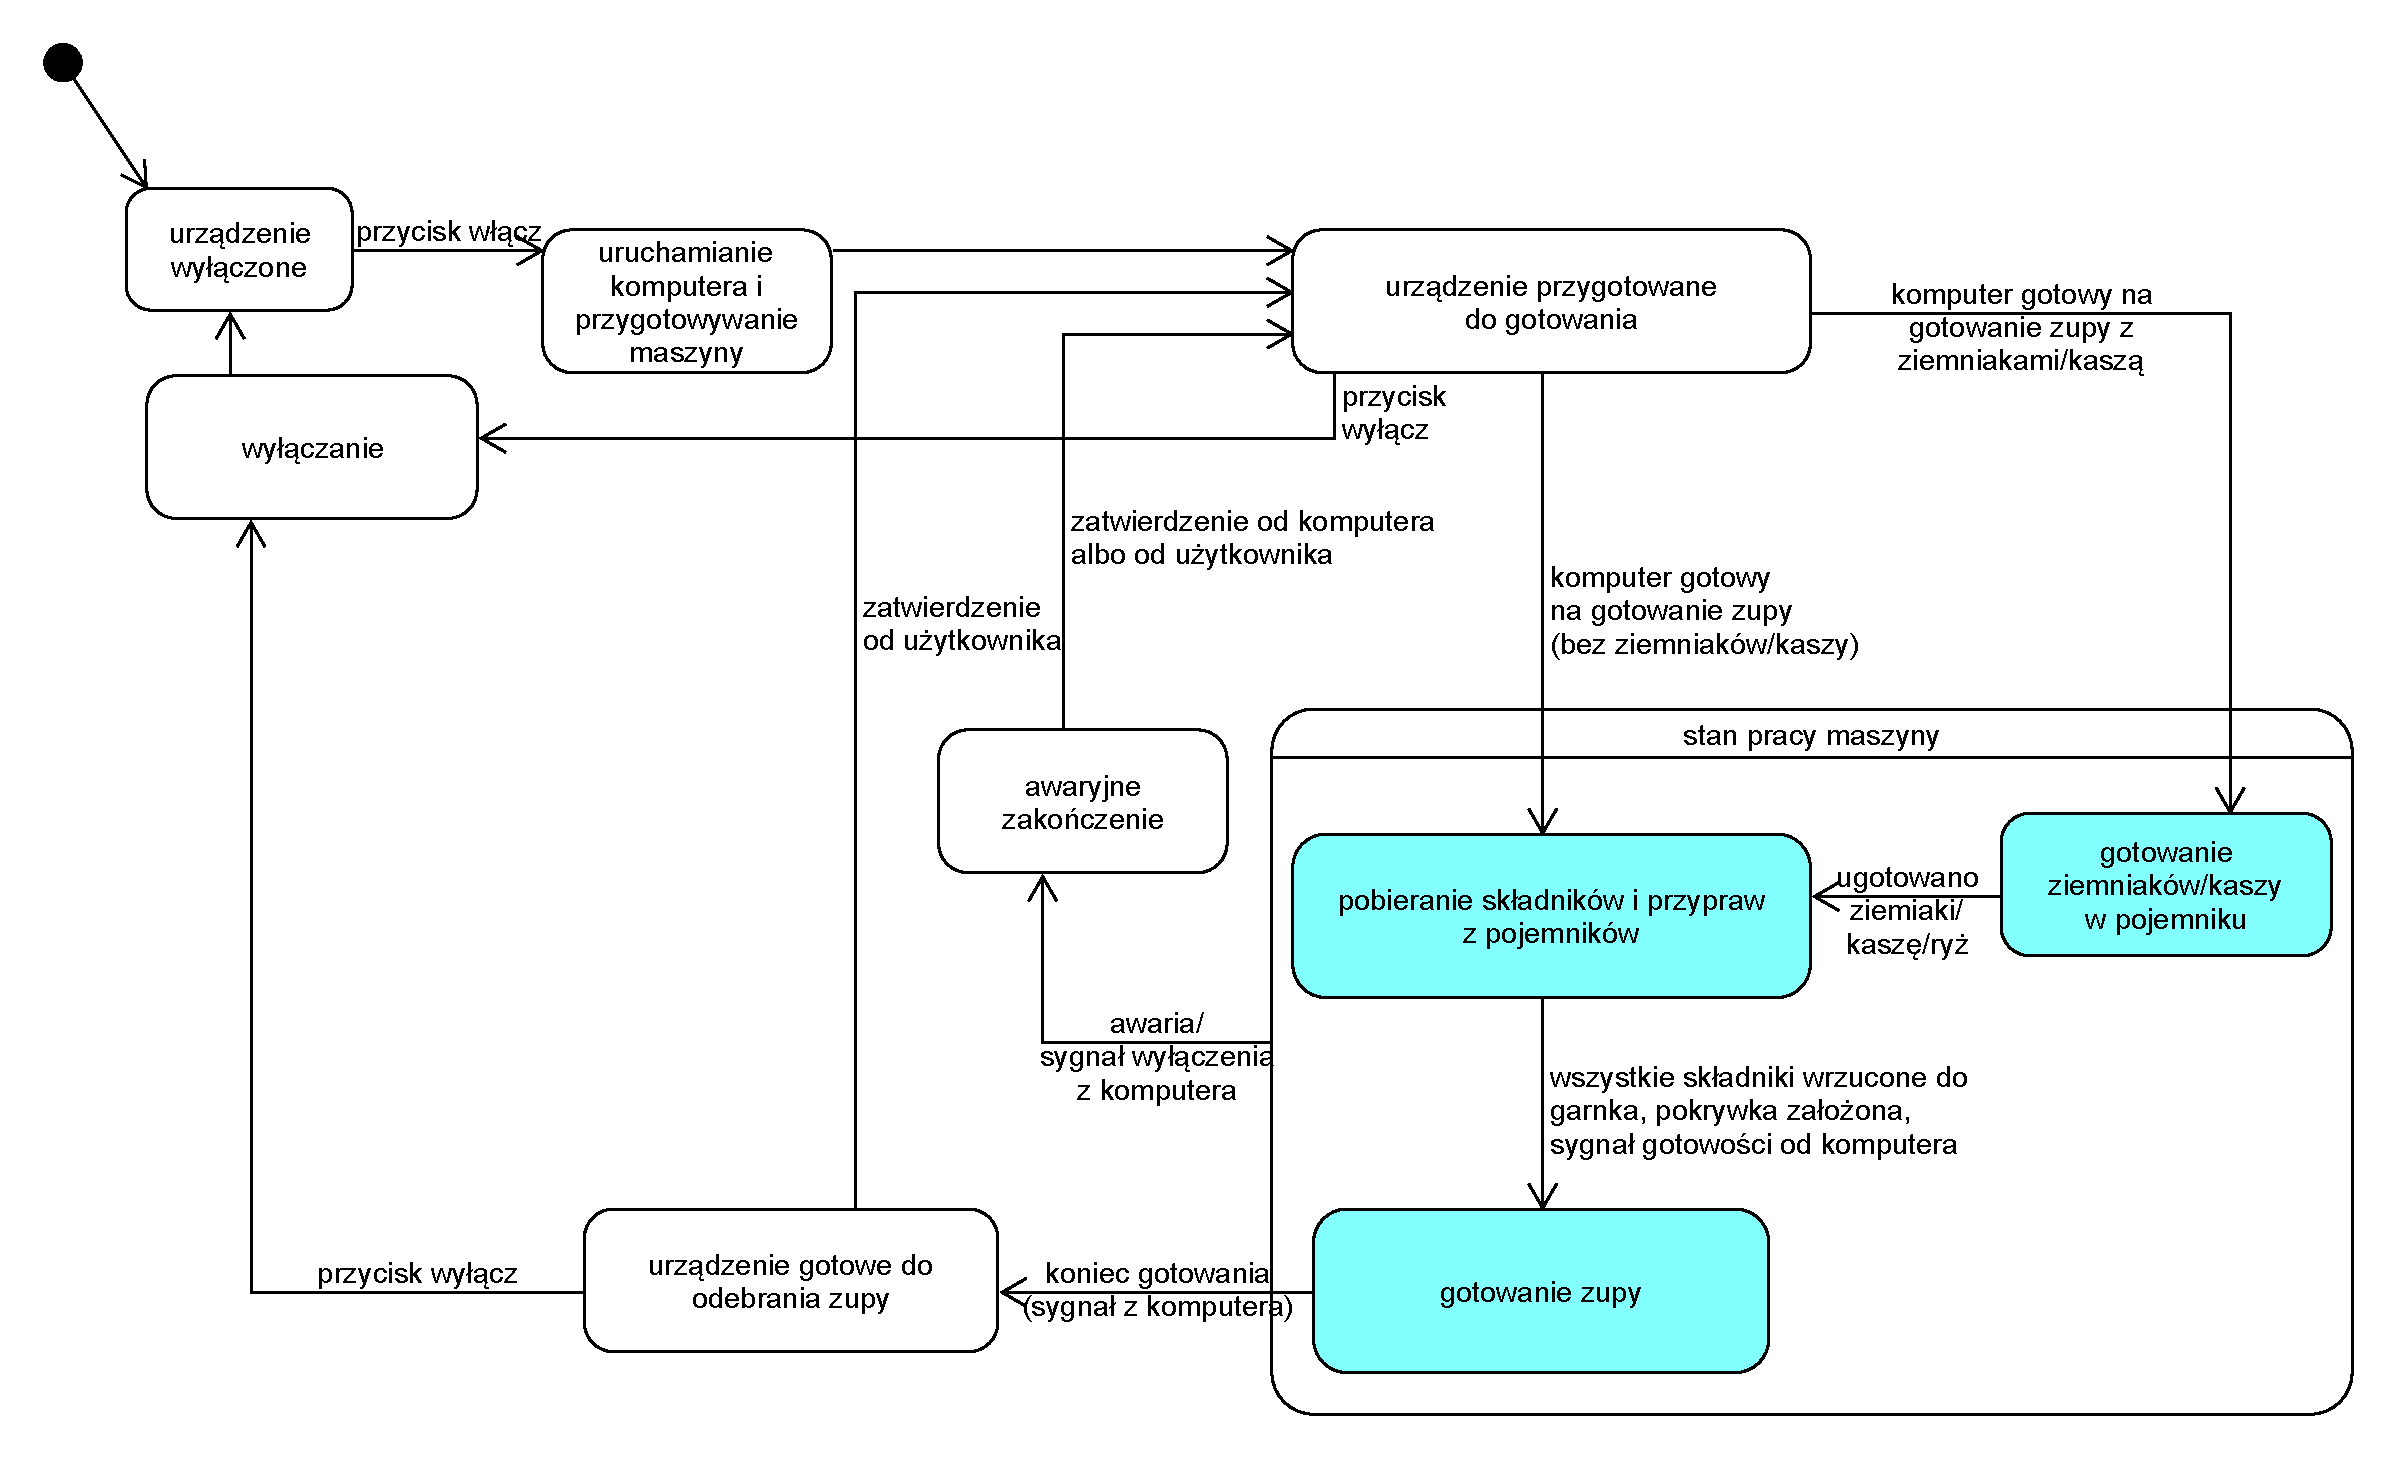
\includegraphics[scale=0.16,width=\textwidth,height=\textheight,keepaspectratio=true]{Diagram-stanow-urzadzenie.pdf}


\newpage
\section{Komponenty systemu}

\subsection{Spis komponentów}
\begin{enumerate}
  \item Zbiornik na wodę
  \item 5 pojemników na składniki z ostrzami
  \item 4 pojemniki na składniki (bez ostrzy)
  \item 5 pojemników na przyprawy
  \item Pojemnik do gotowania ziemniaków/kaszy/makaronu
  \item Pojemnik na wodę po gotowaniu
  \item Stojak na garnek
  \item Komputer - jednostka sterująca
  \item Główny interfejs
  \item Głośnik
  \item Karta sieciowa
  \item System przewodów umożliwiający zasilanie
\end{enumerate}

\subsection{Diagram komponentów}
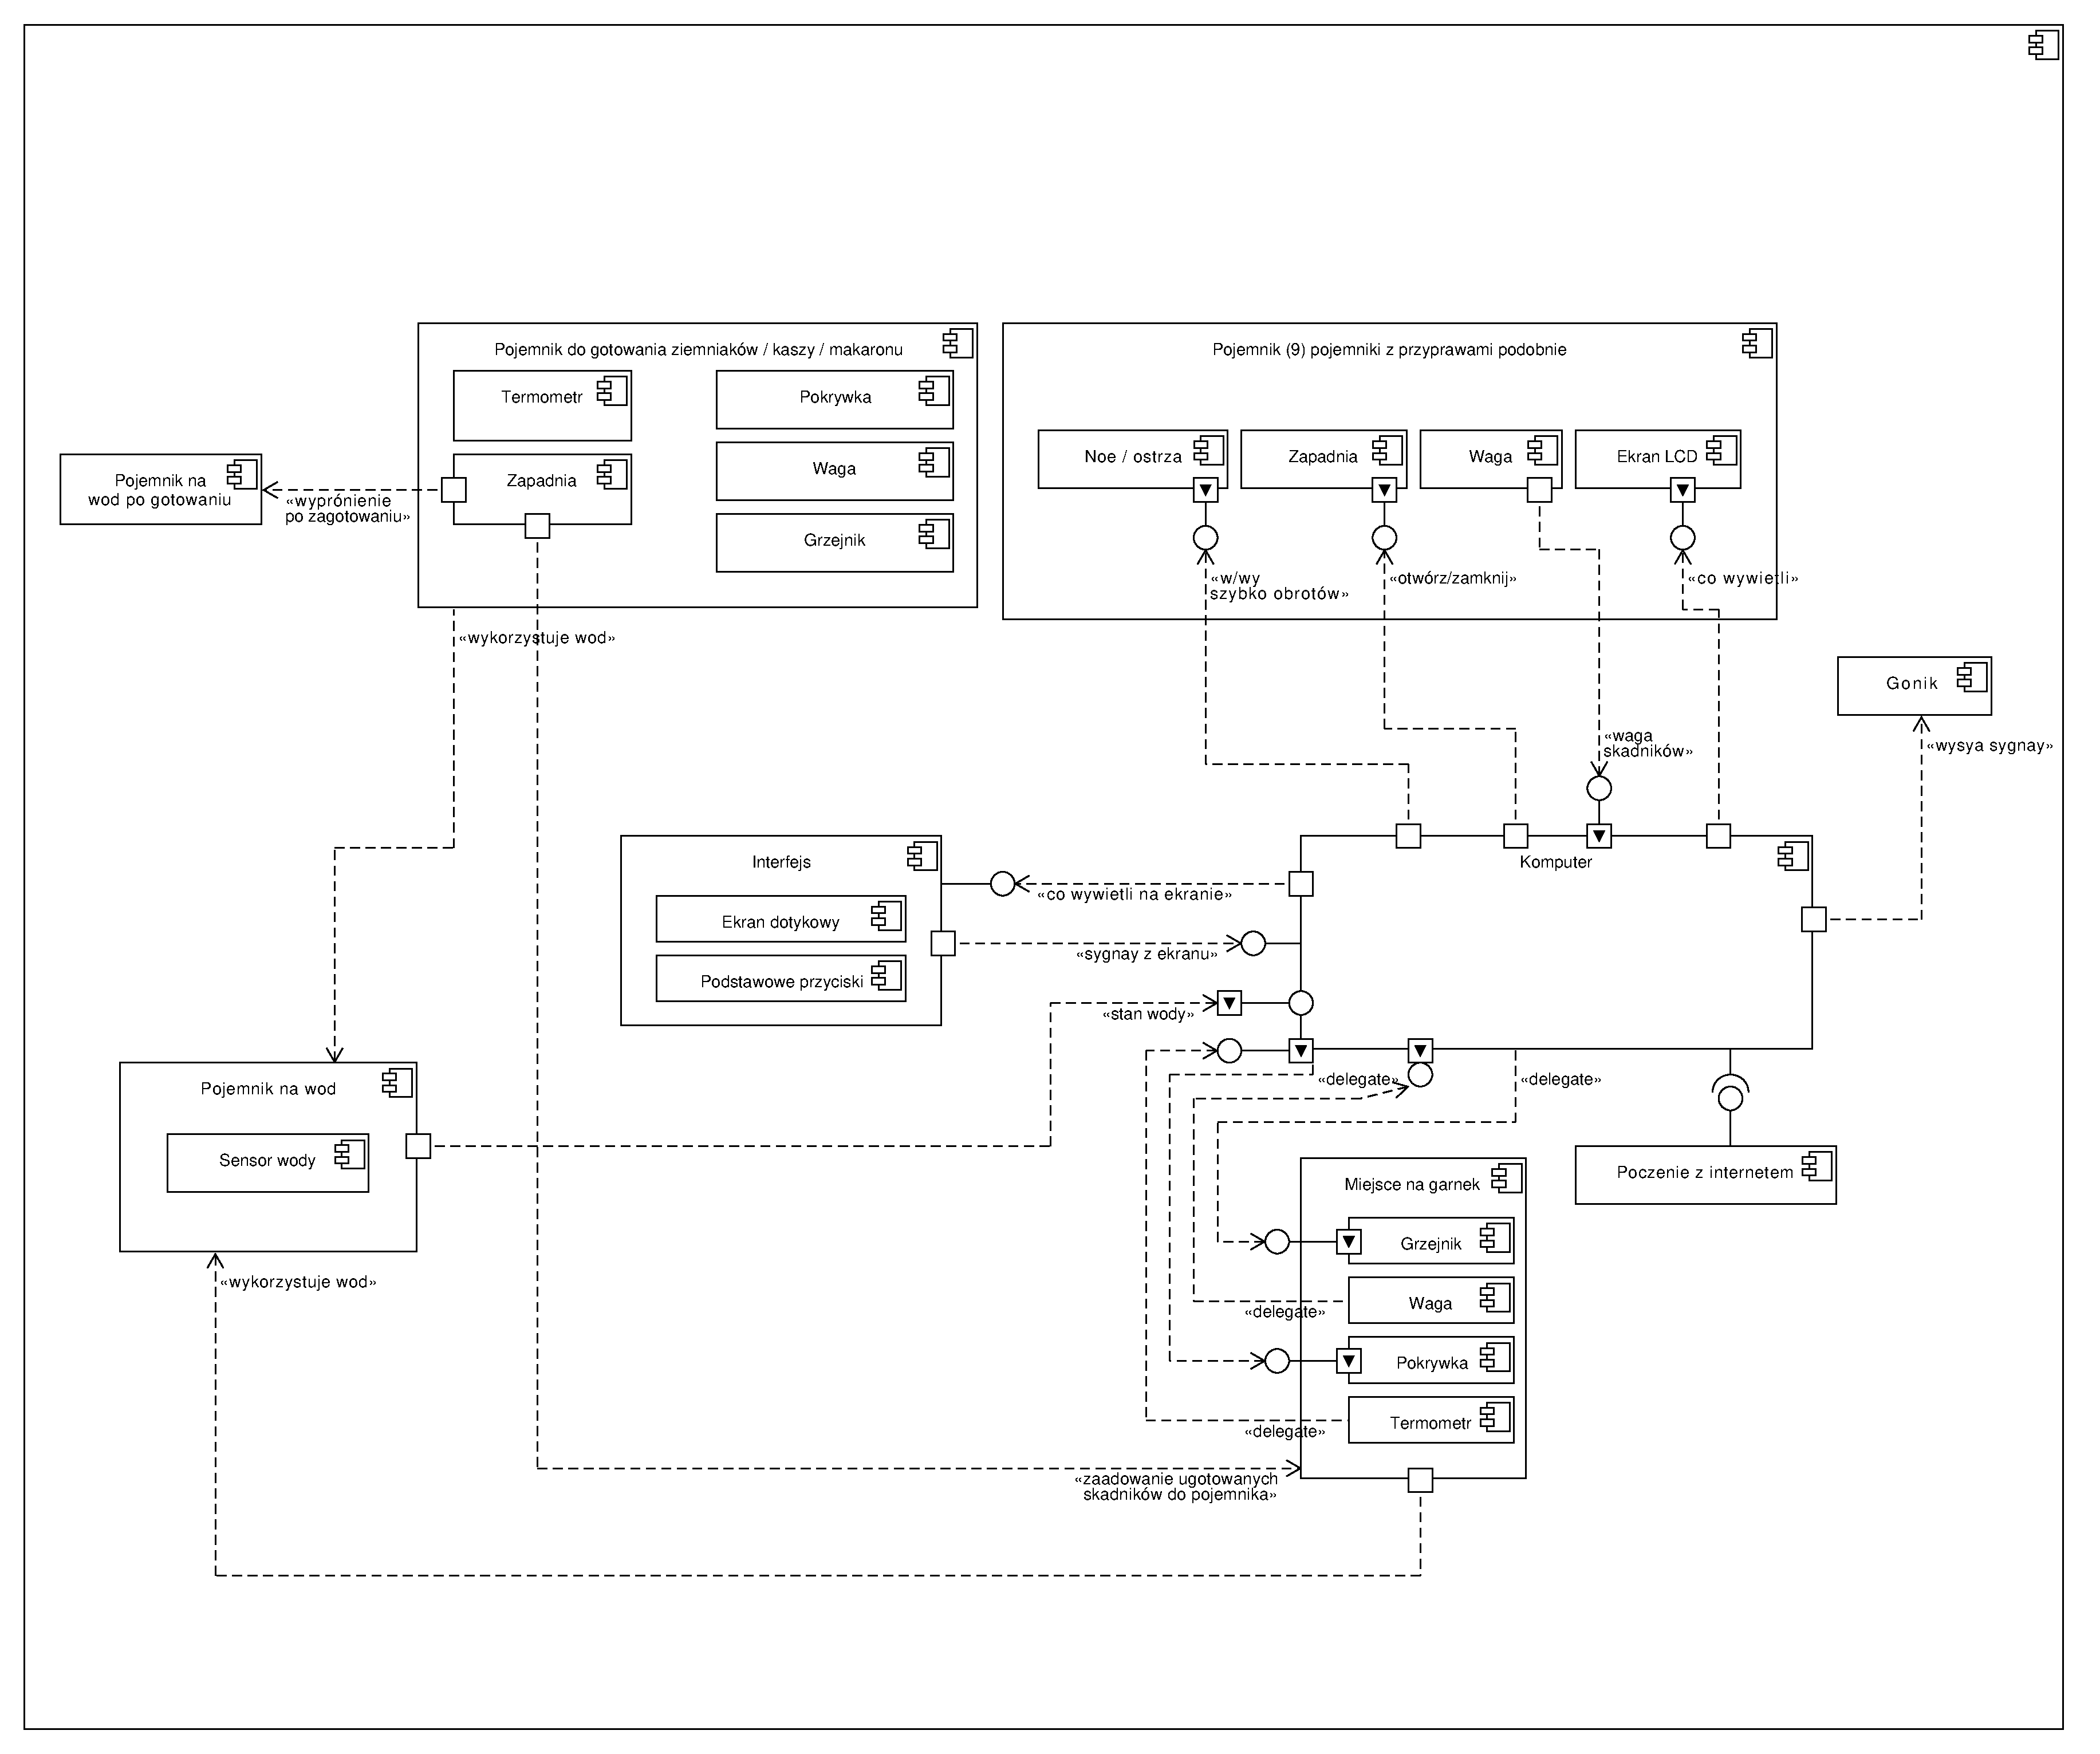
\includegraphics[scale=0.16,width=\textwidth,height=\textheight,keepaspectratio=true]{Diagram_komponentow.pdf}
\newpage

\subsection{Zbiornik na wodę}
\subsubsection{Spis podzespołów komponentu}
\begin{enumerate}
  \item Plastikowy pojemnik o pojemności 10L
  \item Czujnik poziomu wody
  \item Zawory elektromagnetyczne i rynienki do przelewania wody
  \item Połączenie z komputerem
  \item Podłączenie do zasilania
\end{enumerate}

\subsubsection{Dokładniejszy opis budowy i funkcjonalność}
Plastikowy zbiornik na wodę o pojemności 10L. Wewnątrz posiada sensor wody. Posiada połączenie z komputerem w celu wymiany informacji. Zawiera zawory elektromagnetyczne do upuszczania wody i sterowania jej przepływem (do różnych pojemników). Ze względu na korzystanie z prądu posiada połączenie do przewodów zasilających.

\subsubsection{Wykorzystanie i relacje z podzespołami}
Wykorzystuje czujnik poziomu wody do określania aktualnej objętości wody. Używa zaworów i systemu rynienek do napełniania innych pojemników wykorzystujących wodę. 

\subsubsection{Relacje z innymi komponentami}
Pojemnik do gotowania ziemniaków/kaszy/makaronu oraz stojak na garnek wykorzystują wodę z tego komponentu.

\subsubsection{Relacje z użytkownikiem automatu}
Użytkownik uzupełnia pojemnik, jeżeli ten zawiera niewystarczającą ilość wody (informacja podawana na głównym wyświetlaczu automatu).

\subsubsection{Komunikacja z komputerem}
\textbf{Przyjmowane polecenia}: rozkaz odczytu objętości wody, polecenie o napełnienie innych pojemników wodą z tego pojemnika.\\
\textbf{Wysyłane dane}: zmierzona objętość wody w pojemniku, otwarte/zamknięte zawory.

\subsubsection{Awarie i sytuacje wyjątkowe}
\begin{enumerate}
  \item \textbf{Brak wody}\\
Brak wody w pojemniku nie jest sytuacją krytyczną, ale uniemożliwia uruchomienie gotowania. W przypadku braku wody w zbiorniku użytkownik jest o tym informowany, musi uzupełnić wodę w zbiorniku.
  \item \textbf{Uszkodzenie zaworów}\\
W wyniku uszkodzenia zaworów elektromagnetycznych nie ma możliwości napełnienia wodą innych pojemników. Komputer w takiej sytuacji powinien wyświetlić informację o uszkodzeniu zaworów. W najgorszym przypadku awarii zaworów komputer "nie zauważy" awarii zaworów, ale w powodu braku/nadmiaru wody w innych pojemnikach wyświetli informacje o nieprawidłowym działaniu automatu. Automat należy oddać do serwisu.
  \item \textbf{Uszkodzenie przewodów}\\
W przypadku uszkodzenia przewodów zasilających komponent czy uszkodzenia połączenia z komputerem automat musi być oddany do serwisu.
\end{enumerate}



\subsection{Pojemniki na składniki z ostrzami}
\subsubsection{Spis podzespołów komponentu}
Każdy z 5 pojemników z ostrzami zawiera:
\begin{enumerate}
  \item Ostrza
  \item Silnik elektryczny
  \item Górna przykrywka z akrylu
  \item Wsuwana podstawa
  \item Waga z czujnikiem tensometrycznym
  \item Niewielki wyświetlacz LCD
  \item Połączenie z komputerem
  \item Podłączenie do zasilania za pomocą wtyczki
\end{enumerate}

\subsubsection{Dokładniejszy opis budowy i funkcjonalność}
Metalowy, nierdzewny, otwarty z góry pojemnik o wymiarach 10cm $\times$ 7cm $\times$ 10cm. Jest wyposażony w serwomechanizmy wsuwające ruchomą podstawę (do opróżniania pojemnika), kładący akrylową przykrywkę (zabezpieczenie). W środku zawiera zamontowane nierdzewne ostrza (sterowane przez komputer). Posiada silnik elektryczny obracający ostrza, moc 500W. Ma wbudowany w podstawę czujnik tensometryczny, o zakresie miary ciężaru 0-2kg (element wagi). Czujnik jest podłączony do przetwornika analogowo-cyfrowego, który połączony jest z komputerem jako \emph{slave}. Od strony frontowej pojemnik ma wyświetlacz LCD 2x16 znaków. Ze względu na potrzebę wykorzystania prądu pojemnik jest połączony do przewodów zasilających za pomocą wtyczki. Pojemnik jest przystosowany do wyjęcia z urządzenia w celu umycia.
 
\subsubsection{Wykorzystanie i relacje z podzespołami}
Waga jest wykorzystywana do kontrolowania ilości składnikiów. Ostrza są używane do siekania składników na mniejsze części. Akrylowa przykrywka jest zamykana i unieruchamiana na czas siekania składników. Podstawa pojemnika jest wsuwana po procesie siekania, tak aby wszystkie składniki spadły do garnka pod spodem. Wyświetlacz LCD na frontowej ścianie wyświetla informacje o wadze umieszczonych składników.

\subsubsection{Relacje z innymi komponentami}
Przetworzone składniki są usuwane z pojemników dzięki zapadni w podstawie i trafiają do garnka stojącego na stojaku, w którym rozpocznie się gotowanie.

\subsubsection{Relacje z użytkownikiem automatu}
Użytkownik uzupełnia pojemnik odpowiednimi składnikami według instrukcji na ekranie głównym. Po procesie gotowania użytkownik wyjmuje cały pojemnik, usuwa z niego resztki składników i myje przed kolejnym użyciem automatu.

\subsubsection{Komunikacja z komputerem}
\textbf{Przyjmowane polecenia}: rozkaz odczytu wagi składników, rozkaz wyświetlenia informacji na ekranie LCD pojemnika, otwarcie/zamknięcie górnej przykrywki, otwarcie/zamknięcie zapadni, uruchomienie/zatrzymanie ostrzy.\\
\textbf{Wysyłane dane}: otwarty/zamknięty pojemnik, zmierzona waga składników wewnątrz pojemnika.

\subsubsection{Diagram stanów}
\includegraphics[width=\textwidth,height=\textheight,keepaspectratio=true]{Diagram-stanow-pojemnik.pdf}

\subsubsection{Awarie i sytuacje wyjątkowe}
\begin{enumerate}
  \item \textbf{Uszkodzone ostrza/niedziałający silnik}\\
System nie posiada czujników określających uszkodzenie silnika/ostrzy w pojemniku. Jeżeli składniki nie zostaną pokrojone to spadną całe do garnka.
  \item \textbf{Uszkodzenie systemu wysuwania blokady przykrywki}\\
W wyniku uszkodzenia mechanizmu zamknięcia pojemnika zamknięcie zostaje odblokowane, w miarę możliwości otwarte. Komputer dostaje informacje o niezamkniętym pojemniku i wstrzymuje działanie automatu do momentu naprawienia.
  \item \textbf{Awaria wagi}\\
Gdy nastąpi awaria wagi komputer nie otrzyma informacji o wadze składników w pojemniku. Zostanie wyświetlone ostrzeżenie na głównym wyświetlaczu. Proces gotowania zupy może być kontynuowany.
  \item \textbf{Uszkodzenie mechanizmu wysuwania podstawy}\\
W wyniku uszkodzenia mechanizmu otwierania spodu pojemnika zapadnia zostaje otwarta, jeżeli jest to możliwe. Komputer dostaje informacje o usterce.
  \item \textbf{Uszkodzenie wyświetlacza}\\
Ta usterka nie wpływa znacząco na proces użytkowania automatu.
  \item \textbf{Uszkodzenie przewodów}\\
W przypadku uszkodzenia przewodów zasilających komponent czy uszkodzenia połączenia z komputerem automat musi być oddany do serwisu.
\end{enumerate}


\subsection{Pojemniki na składniki (bez ostrzy)}
\subsubsection{Spis podzespołów komponentu}
Każdy z 4 pojemników na składniki (bez ostrzy) zawiera:
\begin{enumerate}
  \item Górna przykrywka z akrylu
  \item Wsuwana podstawa
  \item Waga z czujnikiem tensometrycznym
  \item Niewielki wyświetlacz LCD
  \item Połączenie z komputerem
  \item Podłączenie do zasilania za pomocą wtyczki
\end{enumerate}

\subsubsection{Dokładniejszy opis budowy i funkcjonalność}
Metalowy, nierdzewny, otwarty z góry pojemnik o wymiarach 10cm $\times$ 7cm $\times$ 10cm. Jest wyposażony w serwomechanizmy wsuwające ruchomą podstawę (do opróżniania pojemnika), kładący akrylową przykrywkę (zabezpieczenie). Ma wbudowany w podstawę czujnik tensometryczny, o zakresie miary ciężaru 0-2kg (element wagi). Czujnik jest podłączony do przetwornika analogowo-cyfrowego, który połączony jest z komputerem jako \emph{slave}. Od strony frontowej pojemnik ma wyświetlacz LCD 2x16 znaków. Ze względu na potrzebę wykorzystania prądu pojemnik jest połączony do przewodów zasilających za pomocą wtyczki. Pojemnik jest przystosowany do wyjęcia z urządzenia w celu umycia.
 
\subsubsection{Wykorzystanie i relacje z podzespołami}
Waga jest wykorzystywana do kontrolowania ilości składnikiów. Akrylowa przykrywka jest zamykana i unieruchamiana na czas siekania składników. Wsuwana podłoga jest aby wszystkie składniki spadły do garnka pod spodem przed rozpoczęciem procesu gotowania. Wyświetlacz LCD na frontowej ścianie wyświetla informacje o wadze umieszczonych składników.

\subsubsection{Relacje z innymi komponentami}
Składniki są usuwane z pojemników dzięki wsuwanej podstawie i trafiają do garnka stojącego na stojaku, w którym rozpocznie się gotowanie.

\subsubsection{Relacje z użytkownikiem automatu}
Użytkownik uzupełnia pojemnik odpowiednimi składnikami według instrukcji na ekranie głównym. Po procesie gotowania użytkownik wyjmuje cały pojemnik, usuwa z niego resztki składników i myje przed kolejnym użyciem automatu.

\subsubsection{Komunikacja z komputerem}
\textbf{Przyjmowane polecenia}: rozkaz odczytu wagi składników, rozkaz wyświetlenia informacji na ekranie LCD pojemnika, otwarcie/zamknięcie górnej przykrywki, otwarcie/zamknięcie zapadni.\\
\textbf{Wysyłane dane}: otwarty/zamknięty pojemnik, zmierzona waga składników wewnątrz pojemnika.

\subsubsection{Diagram stanów}
\emph{Diagram stanów taki sam, jak dla pojemnika na składniki z ostrzami.}

\subsubsection{Awarie i sytuacje wyjątkowe}
\emph{Opis awarii i sytuacji wyjątkowych podobny jak dla pojemnika na składniki z ostrzami.}



\subsection{Pojemniki na przyprawy}
\subsubsection{Spis podzespołów komponentu}
Każdy z 5 pojemników na przyprawy zawiera:
\begin{enumerate}
  \item Wsuwana podstawa
  \item Waga z czujnikiem tensometrycznym
  \item Połączenie z komputerem
  \item Podłączenie do zasilania za pomocą wtyczki
\end{enumerate}

\subsubsection{Dokładniejszy opis budowy i funkcjonalność}
Metalowy, nierdzewny, otwarty z góry pojemnik o wymiarach 5cm $\times$ 5cm $\times$ 7cm. Pojemnik nie zawiera przykrywki. Posiada serwomechanizmy wsuwające podstawę. W dolnej części pojemnika mieści się wsuwana podstawa z wbudowaną wagą - czujnikiem tensometrycznym o zakresie miary ciężaru 0-2kg. Czujnik jest podłączony do przetwornika analogowo-cyfrowego, który połączony jest z komputerem jako \emph{slave}. Pojemnik jest połączony do przewodów zasilających za pomocą wtyczki. Pojemnik jest przystosowany do wyjęcia z urządzenia w celu umycia.
 
\subsubsection{Wykorzystanie i relacje z podzespołami}
Waga jest wykorzystywana do kontrolowania ilości przypraw. Celem wsuwanej podstawy jest aby wszystkie składniki spadły do garnka pod spodem przed rozpoczęciem procesu gotowania.

\subsubsection{Relacje z innymi komponentami}
Przyprawy zrzucane pojemnika dzięki wsuwanej podstawie i trafiają do garnka stojącego na stojaku, w którym rozpocznie się gotowanie zupy.

\subsubsection{Relacje z użytkownikiem automatu}
Użytkownik uzupełnia pojemnik odpowiednimi przyprawami według instrukcji na ekranie głównym. Po procesie gotowania zalecane jest aby użytkownik wyczyścił pudełko.

\subsubsection{Komunikacja z komputerem}
\textbf{Przyjmowane polecenia}: rozkaz odczytu wagi składników, otwarcie/zamknięcie zapadni.\\
\textbf{Wysyłane dane}: zmierzona waga przypraw wewnątrz pojemnika.

\subsubsection{Diagram stanów}
\emph{Diagram stanów taki sam, jak dla pojemnika na składniki z ostrzami.}

\subsubsection{Awarie i sytuacje wyjątkowe}
\emph{Opis awarii i sytuacji wyjątkowych podobny jak dla pojemnika na składniki z ostrzami.}


\subsection{Pojemnik do gotowania ziemniaków/kaszy/makaronu}
\subsubsection{Spis podzespołów komponentu}
\begin{enumerate}
  \item Akrylowa przykrywka
  \item Dwie grzałki elektryczne
  \item Termometr
  \item Waga z czujnikiem tensometrycznym
  \item Zawór elektromagnetyczny do spuszczania wody
  \item Zapadnia (na ziemniaki/makaron/kaszę)
  \item Połączenie z komputerem
  \item Podłączenie do zasilania
\end{enumerate}

\subsubsection{Dokładniejszy opis budowy i funkcjonalność}
Pojemnik służy do gotowania ziemniaków/kaszy/makaronu lub innych produktów wymagających zagotowanie. Metalowy, nierdzewny pojemnik o pojemności 2L. Posiada akrylową przykrywkę. Jest wyposażony w serwomechanizmy kładące akrylową przykrywkę (z niewielkim otworem na wydostanie się pary wodnej), otwierające zapadnię. Wewnątrz posiada grzejnik - dwie grzałki elektryczne. Posiada moduł termometru o zakresie pomiarowym od -50\degree C do 290\degree C. Ma wbudowany czujnik tensometryczny, o zakresie miary ciężaru 0-5kg (element wagi). Czujnik jest podłączony do przetwornika analogowo-cyfrowego, który połączony jest z komputerem jako \emph{slave}. Posiada zapadnię.
 
\subsubsection{Wykorzystanie i relacje z podzespołami}
Ma wbudowaną wagę służącą do oszacowania ilości wody przed rozpoczęciem gotowania oraz wagi ziemniaków po włożeniu do pojemnika. Posiada zawory do odlania brudnej wody. Zawiera zapadnię do przeładowania składników do garnka. Za pomocą termometru sprawdza temperaturę wody. Wymaga podłączenia do sieci elektrycznej. Duże zużycie energii ze względu na wykorzystanie grzałek do zagotowania wody.

\subsubsection{Relacje z innymi komponentami}
Ma połączenie ze zbiornikiem na wodę oraz ze zbiornikiem na wodę po gotowaniu. Jest napełniany wodą ze zbiornika na wodę. Gorącą, niezdatną do spożycia wodę wylewa przewodami do pojemnika na wodę po gotowaniu.

\subsubsection{Relacje z użytkownikiem automatu}
Użytkownik wkłada do środka odpowiednie składniki np. makaron, obrane ziemniaki.

\subsubsection{Komunikacja z komputerem}
\textbf{Przyjmowane polecenia}: otwórz/zamknij pokrywkę, uruchom/wyłącz grzejnik, otwórz/zamknij zapadnię, sprawdź temperaturę wody, sprawdź wagę wody/składników\\
\textbf{Wysyłane dane}: temperatura wody, waga.

\subsubsection{Diagram stanów}
\includegraphics[width=\textwidth,height=\textheight,keepaspectratio=true]{Diagram-stanow-pojemnik-na-ziemniaki.pdf}

\subsubsection{Awarie i sytuacje wyjątkowe}
\begin{enumerate}
  \item \textbf{Awaria mechanizmu otwierania zapadni czy kładzenia przykrywki}
W przypadku awarii mechanizmu kładzenia przykrywki, lub uszkodzenia przykrywki, automat kontynuuje gotowanie wody. Natomiast gdy zapadnia na ugotowane składniki nie działa prawidłowo komputer rozpoznaje problem poprzez pomiar wagi zawartości pojemnika po gotowaniu. Wyświetlany jest błąd, sugerowane jest oddanie automatu do serwisu.
  \item \textbf{Nie działające grzałki}
Jeżeli grzałki nie działają, to komputer odkrywa ten problem dzięki sprawdzeniu temperatury wody. Wyświetlany jest błąd, sugerowane jest oddanie automatu do serwisu.
  \item \textbf{Niesprawny termometr}
W momencie gdy moduł termometru jest niesprawny komputer nie otrzymuje odpowiedzi od komponentu na temat temperatury wody. W tym przypadku wyświetlany jest błąd i sugerowane jest oddanie automatu do naprawy w serwisie.
  \item \textbf{Uszkodzenie przewodów}\\
W przypadku uszkodzenia zaworów odprowadzających brudną wodę, komputer dowiaduje się o tym sprawdzając wagę zawartości pojemnika po poleceniu otwarcia zaworów. Jeżeli waga jest nieprawidłowa przerywany jest proces gotowania. Wyświetlany jest komunikat błędu. Należy oddać urządzenie do naprawy.
  \item \textbf{Uszkodzenie przewodów}\\
W przypadku uszkodzenia przewodów zasilających komponent czy uszkodzenia połączenia z komputerem automat musi być oddany do serwisu.
\end{enumerate}




\subsection{Pojemnik na wodę po gotowaniu}
\subsubsection{Spis podzespołów komponentu}
\begin{enumerate}
  \item Sensor wody - czujnik pływakowy
  \item Połączenie z komputerem
  \item Podłączenie do zasilania
\end{enumerate}

\subsubsection{Dokładniejszy opis budowy i funkcjonalność}
Duży plastikowy pojemnik o pojemności 9L umieszczony na dole urządzenia. Pojemnik zawiera sensor wody złożony z czujnika pływakowego poziomu cieczy. Jest połączony do zasilania oraz do komputera.
 
\subsubsection{Wykorzystanie i relacje z podzespołami}
Pojemnik zawiera prosty sensor wody umieszczony w górnej części. Jeżeli pojemnik jest prawie pełny sensor to wykryje i będzie w stanie poinformować o tym komputer główny automatu.

\subsubsection{Relacje z innymi komponentami}
Do tego pojemnika spływa niezdatna do picia gorąca woda po gotowaniu.

\subsubsection{Relacje z użytkownikiem automatu}
Użytkownik opróżnia pojemnik, gdy ten jest pełny. Zostanie o tym poinformowany poprzez komunikat na ekranie głównym.

\subsubsection{Komunikacja z komputerem}
\textbf{Przyjmowane polecenia}: rozkaz uruchomienia sensora wody i sprawdzenia poziomu wody.\\
\textbf{Wysyłane dane}: czy woda osiągnęła określony poziom krytyczny.

\subsubsection{Awarie i sytuacje wyjątkowe}
\begin{enumerate}
  \item \textbf{Awaria sensora wody }\\
W przypadku nieprawidłowego działania sensora wody komputer powinien dostać nieprawidłową odpowiedź. Wtedy wyświetlane jest ostrzeżenie o możliwości przepełnienia pojemnika. Użytkownik może kontynuować korzystanie z automatu, ale musi samemu sprawdzać stan napełnienia pojemnika.
  \item \textbf{Uszkodzenie przewodów}\\
W przypadku uszkodzenia przewodów zasilających komponent czy uszkodzenia połączenia z komputerem automat musi być oddany do serwisu.
\end{enumerate}



\subsection{Stojak na garnek}
\subsubsection{Spis podzespołów komponentu}
\begin{enumerate}
  \item Grzejnik indukcyjny
  \item Waga z czujnikiem tensometrycznym
  \item Pokrywka
  \item Termometr
  \item Połączenie z komputerem
  \item Połączenie do zasilania
\end{enumerate}

\subsubsection{Dokładniejszy opis budowy i funkcjonalność}
Metalowy stojak na garnek, który jest w zestawie z automatem. Stojak ma wbudowany induktor do grzejnika, moc 2300 W, połączony z komputerem, który steruje mocą induktora (przez przetwornik analogowo cyfrowy). Posiada czujnik tensometryczny, o zakresie miary ciężaru 0-15kg (element wagi). Serwomechanizm do nałożenia pokrywki na garnek. Posiada wentylator do grzejnika. Czujnik jest podłączony do przetwornika analogowo-cyfrowego, który połączony jest z komputerem jako \emph{slave}. Posiada moduł termometru o zakresie pomiarowym od -50\degree C do 290\degree C. Jest wyposażony w szklaną przykrywkę na garnek. Ma wentylator do grzenika.
 
\subsubsection{Wykorzystanie i relacje z podzespołami}
Waga służy do sprawdzenia czy na stojaku jest umieszczony garnek. Termometr służy do kontroli temperatury wody, jako że niektóre zupy powinny być gotowane w niewrzącej wodzie. Wszystkie podzespoły są kontrolowane przez komputer główny.

\subsubsection{Relacje z innymi komponentami}
Posiekane składniki oraz przyprawy spadają do garnka na stojaku z pojemników przed rozpoczęciem procesu gotowania. Garnek na stojaku zostaje wypełniony wodą ze zbiornika na wodę.

\subsubsection{Relacje z użytkownikiem automatu}
Użytkownik kładzie garnek przed uruchomieniem urządzenia. Po gotowaniu zdejmuje garnek z zupą. Po opróżnieniu garnka użytkownik myje garnek i ponownie kładzie go na stojak.

\subsubsection{Komunikacja z komputerem}
\textbf{Przyjmowane polecenia}: otwórz/zamknij szklaną pokrywkę, uruchom/wyłącz grzejnik indukcyjny, sprawdź czy garnek jest położony na stojaku (waga), sprawdź temperaturę.\\
\textbf{Wysyłane dane}: aktualna temperatura, czy garnek znajduje się na stojaku.

\subsubsection{Awarie i sytuacje wyjątkowe}
\begin{enumerate}
  \item \textbf{Brak położonego garnka na stojaku}\\
Jeżeli użytkownik nie postawił garnka na stojaku, co jest sprawdzane dzięki pobraniu informacji o wadze, automat zatrzymuje pracę i czeka na postawienie garnka.
  \item \textbf{Awaria grzejnika}\\
W przypadku gdy grzejnik nie działa komputer dowiaduje się o tym poprzez analizowanie temperatury. Wyświetla informację o awarii grzejnika. Sugerowane jest oddanie automatu do naprawy.
  \item \textbf{Uszkodzony mechanizm kładzenia przykrywki na garnek, niepołożona przykrywka}\\
Przykrywka na garnku nie jest niezbędna, ale zalecana. Uszkodzony mechanizm nakładania przykrywki na garnek nie uniemożliwia korzystania z automatu, ale inne elementy automatu mogą być narażone na uszkodzenie przez parę wodną.
  \item \textbf{Niesprawny termometr}
W momencie gdy moduł termometru jest niesprawny komputer nie otrzymuje odpowiedzi od komponentu na temat temperatury wody. W tym przypadku wyświetlany jest błąd. Może to być przyczyną wygotowania zupy. Zalecana jest naprawa.
  \item \textbf{Uszkodzenie przewodów}\\
W przypadku uszkodzenia przewodów zasilających komponent czy uszkodzenia połączenia z komputerem automat musi być oddany do serwisu.
\end{enumerate}




\subsection{Komputer}
Opis i działanie komputera jako głównej jednostki obliczeniowej i sterującej znajduje się w osobnym rozdziale.

\subsection{Główny interfejs}
\subsubsection{Spis podzespołów komponentu}
\begin{enumerate}
  \item Ekran dotykowy
  \item Przycisk Start
  \item Przycisk Góra
  \item Przycisk Dół
  \item Przysisk Wtecz
  \item Przycisk Wyłącz/Włącz automat
  \item Połączenie z komputerem
  \item Połączenie do zasilania
\end{enumerate}

\subsubsection{Dokładniejszy opis budowy i funkcjonalność}
Główny interfejs to ekran oraz wbudowane przyciski. PDA - TM7000 -  Ekran dotykowy, seria PDA, LCD kolorowy, 800 x 480, działa we współpracy z procesorem Atmel AVR. Ustawiony jest w pozycji wertykalnej. Na dolnej części obudowy ekranu znajdują się przyciski, takie jak w spisie powyżej.
 
\subsubsection{Wykorzystanie i relacje z podzespołami}
Przyciski na ekranie służą wysyłaniu sygnałów do komputera. Celem ekranu dotykowego jest ergonomiczność i prostota korzystania z automatu dla użytkownika.

\subsubsection{Relacje z innymi komponentami}
Interfejs nie ma połączenia z innymi komponentami, oprócz komputera.

\subsubsection{Relacje z użytkownikiem automatu}
Użytkownik uruchamia automat za pomocą przycisku włącz/wyłącz. Użytkownik przegląda i wybiera przepis za pomocą przycisków i ekranu dotykowego. Użytkownik kieruje się instrukcjami wyświetlanymi na ekranie.

\subsubsection{Komunikacja z komputerem}
Przyjmowane polecenia: co wyświetlić na ekranie.\\
Wysyłane dane: sygnały z interfejsu i wybory użytkownika.

\subsubsection{Diagram stanów}
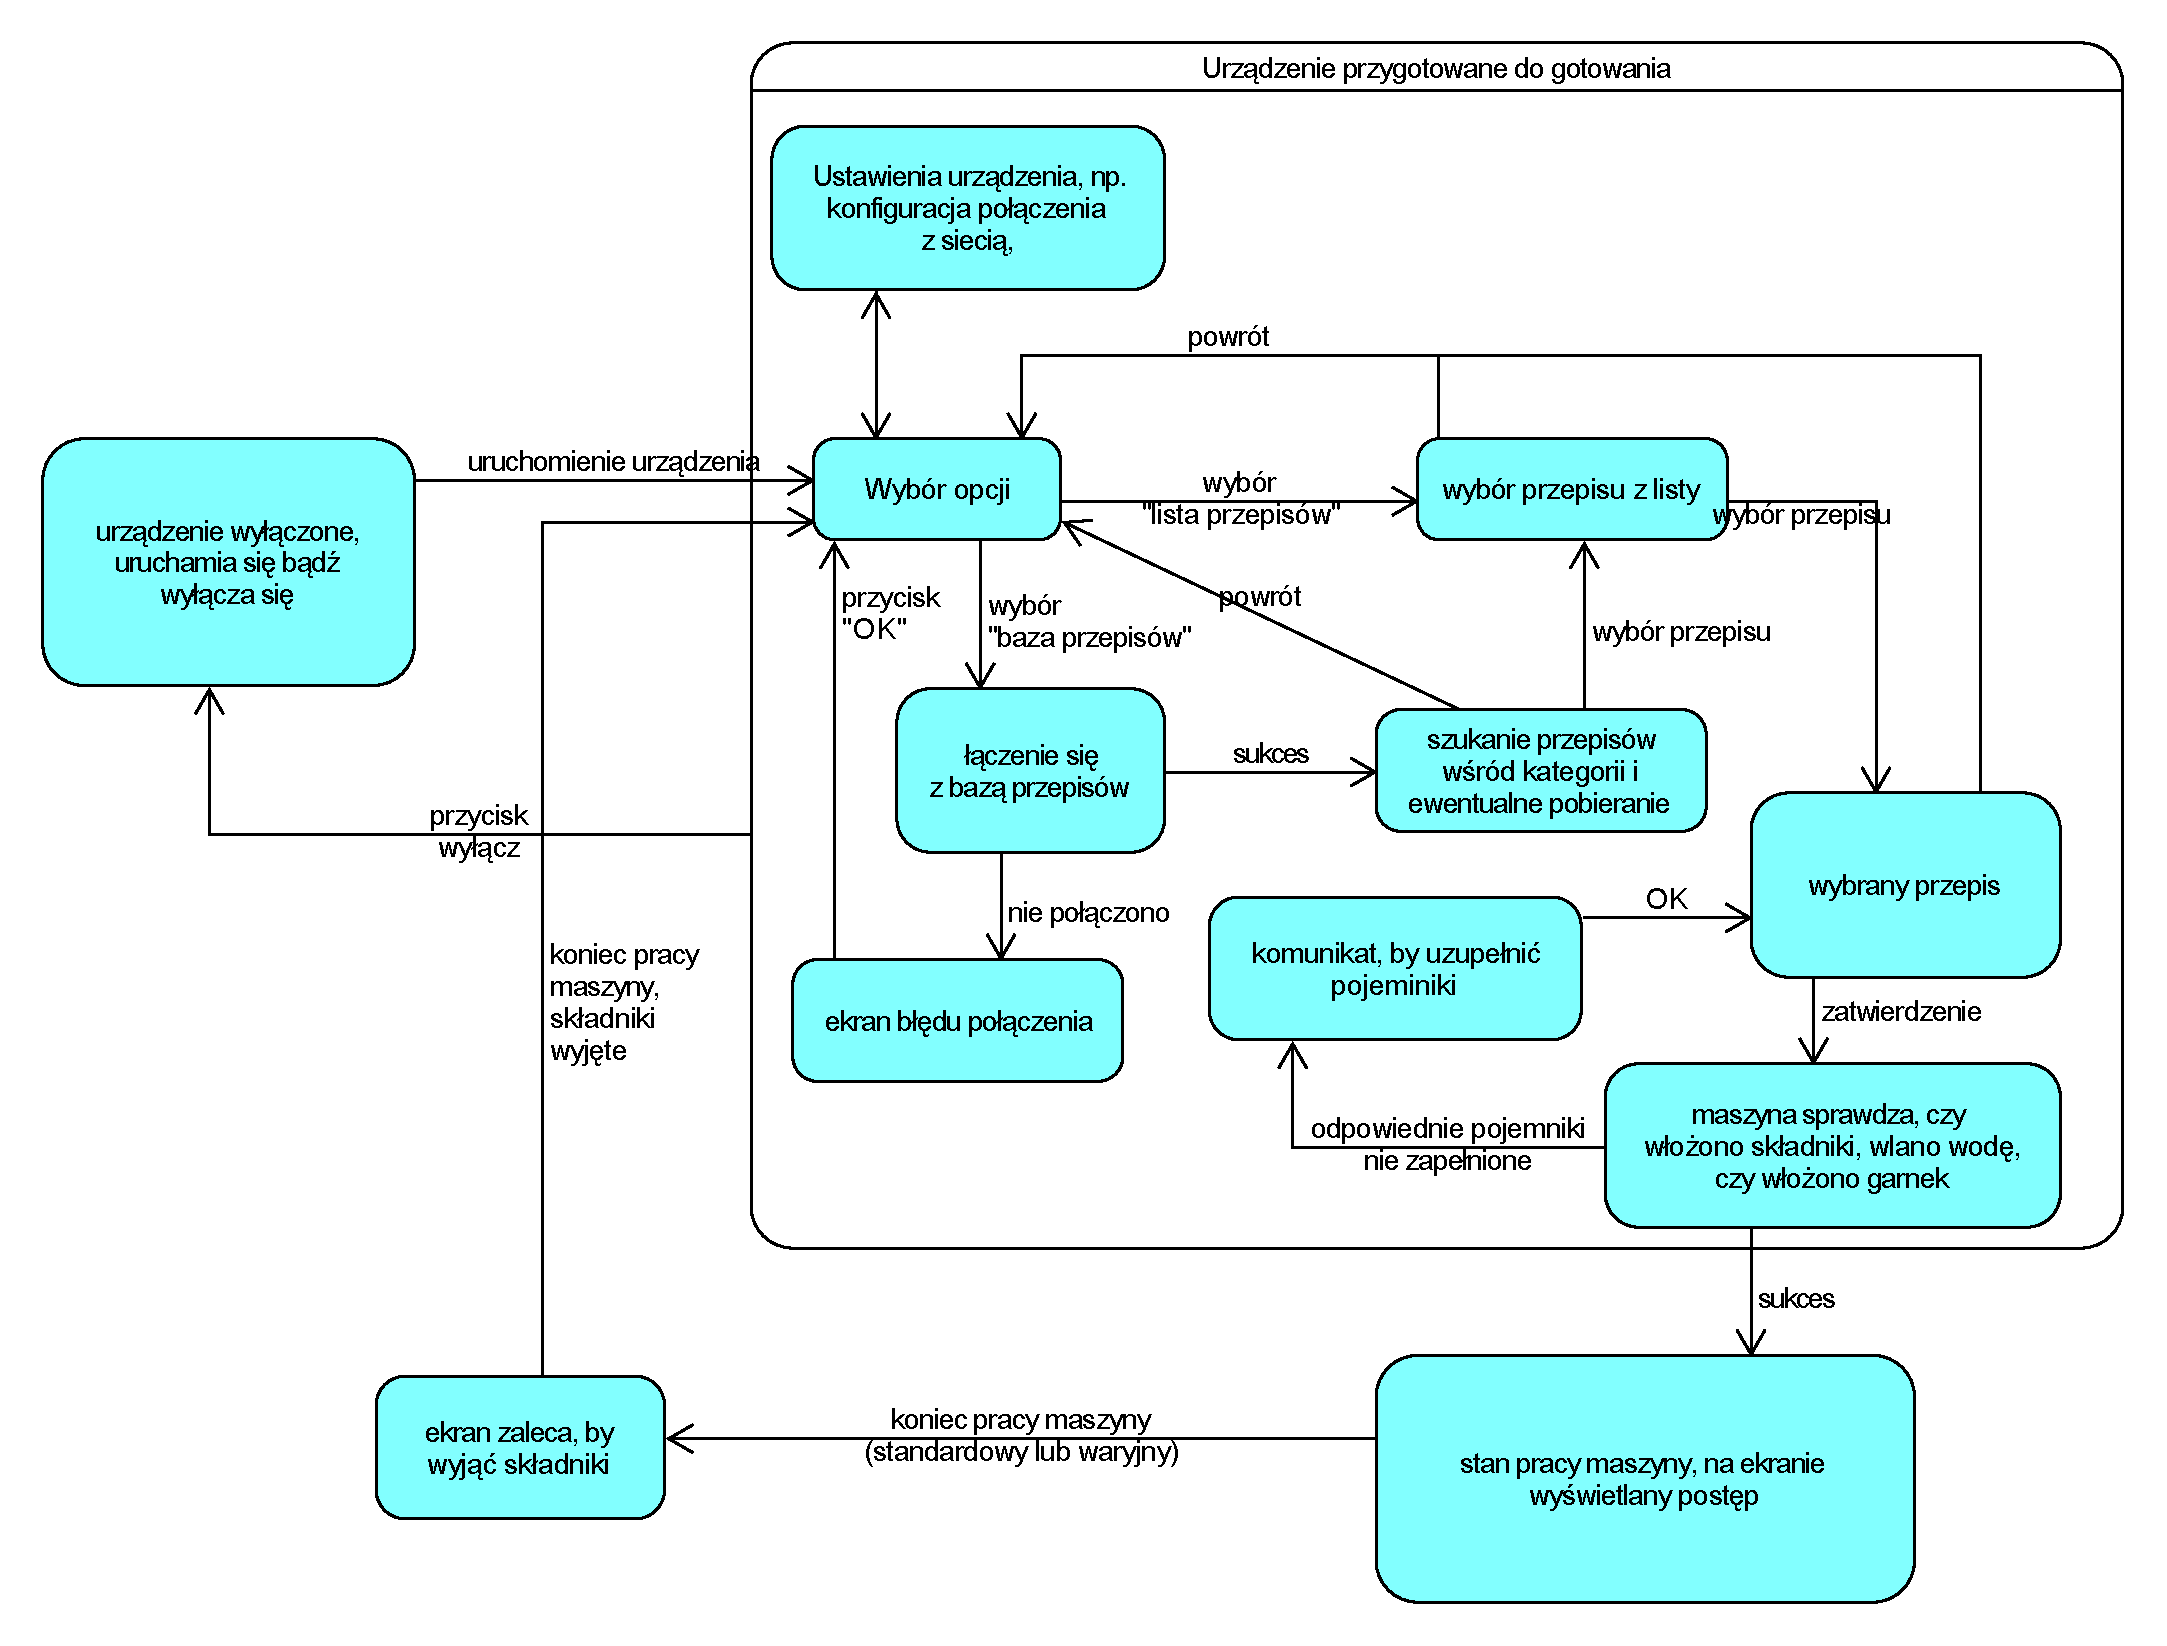
\includegraphics[width=\textwidth,height=\textheight,keepaspectratio=true]{Diagram-stanow-interfejs.pdf}\\
\small
Opis niektórych stanów:
\begin{itemize}

\item \textbf{Urządzenie wyłączone, uruchamia się bądź wyłącza się} - ekran dotykowy jest zablokowany, po uruchomieniu komputera, przechodzi w stan wyboru opcji
\item \textbf{Wybór opcji} - na ekranie dotykowym wywietlają się następujące opcje: \emph{lista przepisów}, \emph{internetowa baza przepisów}, \emph{ustawienia i konfiguracja}, \emph{wyłącz urządzenie}, wywietlają się także ostrzeżenia, np. \emph{brak wody w pojemniku}, \emph{pojemniki na brudną wodę zapełniony} 
\item \textbf{Ustawienia urządzenia...} - na ekranie dotykowym wywietlają się ustawienia urządzenia. Są to m.in.: \emph{Połączenie Wi-Fi}, \emph{Ustawienia ekranu}, \emph{Ustawienia daty i godziny}.
\item \textbf{wybór przepisu z listy} - maszyna ładuje przepisy z karty SD. Listę można przesuwać oraz wybierać z niej przepisy. Można zmieniać przepisy przyciskami góra/dół. Można także szukać przepis wg. nazwy (za pomocą uproszczonej klawiatury na ekranie)
\item \textbf{szukanie przepisów wród kategorii i ewentualne pobieranie} - po poprawnym połączeniu się z bazą internetową, można szukać przepisy na zupy wg. kategorii, wywietlać informacje w nich zawarte oraz pobierać do pamięci urządzenia. 
\item \textbf{wybrany przepis} - wywietla się przepis i informacje o nim (m.in. składniki, czas gotowania). Można wrócić do poprzedniej listy, rozpocząć przygotowanie do gotowania, bądź usunąć przepis z listy.
\item \textbf{maszyna sprawdza czy włożono składniki...} - sprawdzanie, czy maszyna jest gotowa na rozpoczęcie gotowania
\item \textbf{stan pracy maszyny} - ekran nie ma możliwosci interakcji z użytkownikiem, na ekranie wyswietlany jest postęp. Możliwe jest awaryjne zakończenie pracy, przez dwukrotne wcisnięcie przycisku "wyłącz".
\item \textbf{ekran zaleca, by wyjąć składniki} - koniec gotowania, interfejs przechodzi do stanu "wybór opcji", gdy garnek z zupą zostanie wyjęty lub zostanie nacisnięty odpowiedni przycis na ekranie.
%następuje sprawdzenie następujących warunków: czy włożono odpowiednią ilosć wszystkich składników, czy zbiornik na wodę zawiera odpowiednią ilosć wody, czy 

\end{itemize}

\normalsize

\subsubsection{Awarie i sytuacje wyjątkowe}
. . . To Do . . .



\subsection{Głośnik}
\subsubsection{Spis podzespołów komponentu}
\begin{enumerate}
  \item Głośnik
  \item Karta dźwiękowa
  \item Połączenie z komputerem
  \item Połączenie do zasilania
\end{enumerate}

\subsubsection{Dokładniejszy opis budowy i funkcjonalność}
Prosty głośnik z wbudowaną kartą dźwiękową. Odtwarza wbudowaną melodię na polecenie komputera.
 
\subsubsection{Wykorzystanie i relacje z podzespołami}
Karta dźwiękowa to obowiązkowy element głośnika. Posiada wbudowaną prostą melodię. Jest połączony z komputerem oraz jest połączony do zasilania.

\subsubsection{Relacje z innymi komponentami}
Głośnik nie ma połączenia z innymi komponentami, oprócz komputera.

\subsubsection{Relacje z użytkownikiem automatu}
Użytkownik słyszy sygnał zakończenia gotowania.


%\subsubsection{Wykorzystane podzespoły}
%\begin{itemize}
%\item 
%\end{itemize}

\subsubsection{Komunikacja z komputerem}
\textbf{Przyjmowane polecenia}: uruchom dźwięk.\\
\textbf{Wysyłane dane}: brak.

%\subsubsection{Diagram stanów}
%. . . To Do . . .

\subsubsection{Awarie i sytuacje wyjątkowe}
\begin{enumerate}
  \item \textbf{Uszkodzenie głośnika lub karty dźwiękowej}\\
Ta usterka nie wpływa bardzo na działanie automatu. Użytkownik nie zostanie poinformowany dźwiękowo o skończeniu gotowania.
\end{enumerate}

\section{Komputer}

\subsection{Specyfikacja komputera}
.. Grzesiek To Do ok? x) ..
Arduino?
Jaki system
Jakie podzespoły, karta sieciowa (?)
Nie mam pojecia

\subsection{Komunikacja między komputerem a komponentami}
Komputer komunikuje się z pozostałymi komponentami protokołem I$^2$C, gdzie urządzeniem typu \emph{master} jest komputer, a urządzeniami typu \emph{slave} są czujniki i urządzenia wykonawcze.

\section{Aplikacja mobilna}
\subsection{Konfiguracja aplikacji}
Aplikacja mobilna jest dostępna za darmo na system Android oraz iOS. Użytkownik posiadający automat "sparowuje" z nim aplikację w urządzeniu mobilnym. Ustawia też 8-znakowe hasło, które wymagane jest do uwierzytelnienia.
\subsection{Zdalne uruchamianie procesu gotowania}
Aplikacja mobilna służy przede wszystkim do zdalnego uruchamiania gotowania w urządzeniu. Po zalogowaniu w aplikacji użytkownik może zdalnie uruchomić gotowanie zupy. Można ustawić start gotowania na określoną godzinę lub ustawić opóźnienie np. zacznij gotowanie za 10 minut. Wymagany jest dostęp do internetu.
\subsection{Edytor przepisów}
Aplikacja posiada także możliwość tworzenia i modyfikacji przepisów a następnie wysyłania na serwer a następnie do automatu w formacie JSON. Można również wysłać przepis do serwisu z przepisami, który po zaakceptowaniu przez administrację będzie widoczny przez wszystkich użytkowników na stronie internetowej.

\end{document}
